% Define the page style
\fancypagestyle{chapterstyle}{
   \fancyhead[L]{\nouppercase{\rightmark}}
   \fancyhead[R]{Projet de fin d'etudes 2023-2024}
   \fancyfoot[C]{\vspace{20pt}\thepage} % Adjust the vertical space here
   \setlength{\headheight}{20pt}
   \setlength{\footskip}{30pt} % Adjust the value as needed
}


\chapter{Conception de la solution}
\pagestyle{chapterstyle}

\newpage
\vspace{1cm}

\section{Introduction}
% Ce chapitre détaille la conception de notre solution. Après avoir défini les 
% besoins et les cas d'utilisation, nous utiliserons des maquettes 
% pour visualiser l'interface utilisateur, des diagrammes de séquence 
% pour illustrer les interactions dynamiques entre les composantes 
% de l'application et des diagrammes de classes pour structurer les 
% éléments et leurs relations. Cette étape assure une mise en œuvre 
% cohérente et efficace, intégrant toutes les exigences identifiées.
% Ce chapitre détaille la conception de notre solution. 
% Après avoir spécifié les besoins, nous avons mis en place des maquettes pour bien illustrer ces besoins. 
% Puis dans le cadre d'une conception générale,
% nous avons conçu une architecture pour notre solution. 
% Par la suite, nous avons conçu le diagramme de classe 
% et les diagrammes de séquence.

Ce chapitre détaille la conception de notre solution. Après avoir spécifié 
les besoins, nous avons créé des maquettes pour illustrer 
ces exigences. Ensuite, dans le cadre d'une conception générale, nous avons 
élaboré une architecture pour notre solution. Par la suite, nous avons 
conçu le diagramme de classes ainsi que les diagrammes de séquence.


\section{Maquettes}
Le design UX/UI est un élément principal de notre projet, 
car il vise à aligner les objectifs du client (entreprise 4D) et ses attentes avec 
le travail qui va être réalisé par la suite.
\newline
Dans notre situation, nous avons converti les besoins fonctionnels du système 
en maquettes. Cela nous a permis de préparer l'interface globale 
avant d'entrer dans la phase de développement. Ensuite, 
nous avons sollicité les retours du client 
afin d'améliorer encore notre application.
\newline
% \vspace{4cm}



\begin{figure}[htbp]
   \centering
   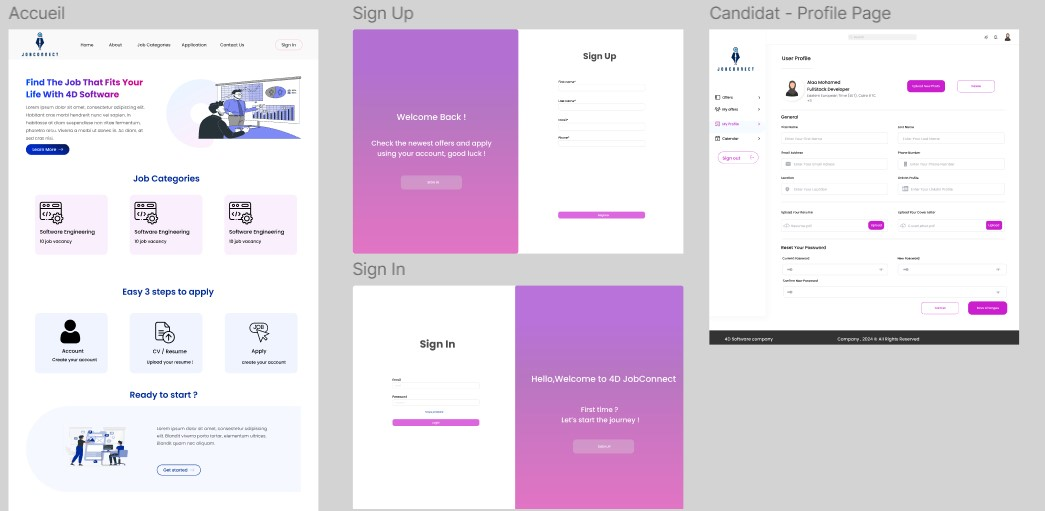
\includegraphics[scale=0.8]{Images/1.jpg} % Replace with the actual filename of the IBM logo image
   \caption{Maquettes Authentification et Profile}
   \label{fig:maquette1}
\end{figure}
% \vspace{1cm}
\vspace{4cm}
\begin{figure}[htbp]
   \centering
   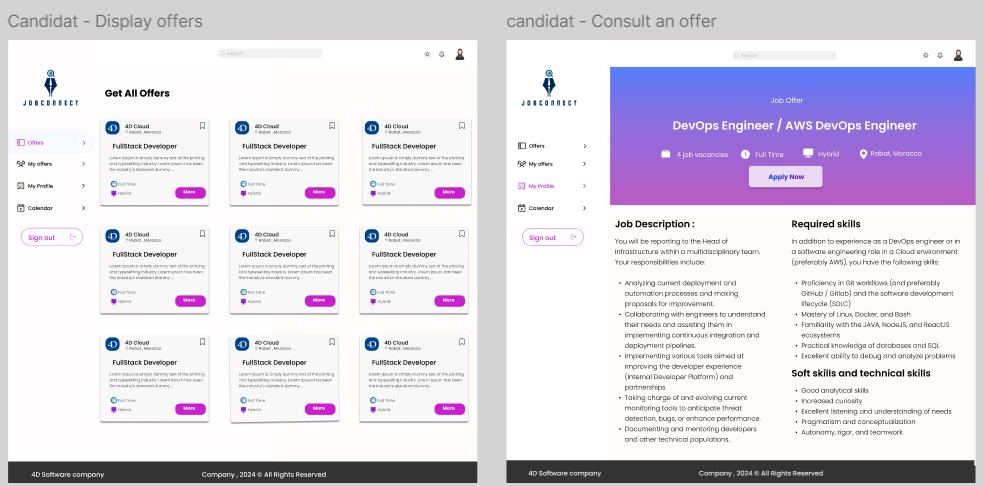
\includegraphics[scale=0.8]{Images/2.jpg} 
   \caption{Maquettes Offres}
   \label{fig:maquette2}
\end{figure}

\begin{figure}[htbp]
   \centering
   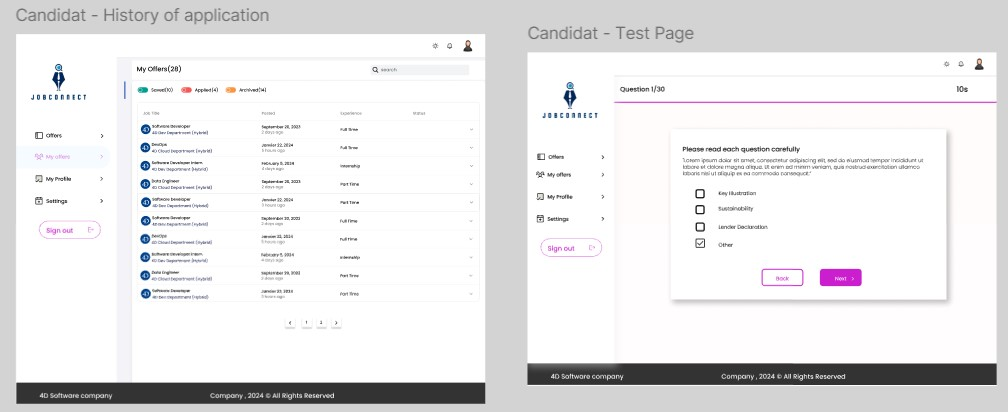
\includegraphics[scale=1]{Images/3.jpg} 
   \caption{Maquettes historique de candidature et test}
   \label{fig:maquette3}
\end{figure}

\begin{figure}[htbp]
   \centering
   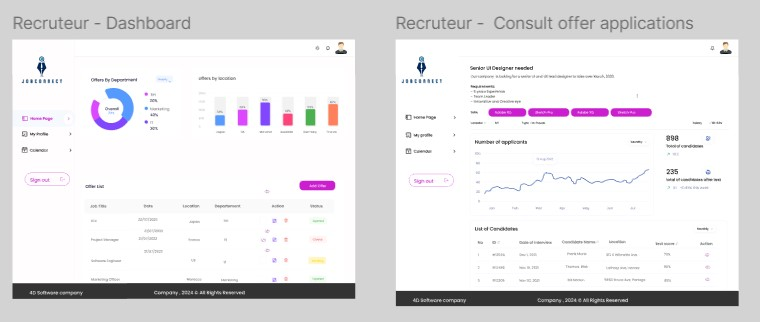
\includegraphics[scale=1.4]{Images/4.jpg} 
   \caption{Maquettes Dashboard recruteur}
   \label{fig:maquette4}
\end{figure}

\begin{figure}[htbp]
   \centering
   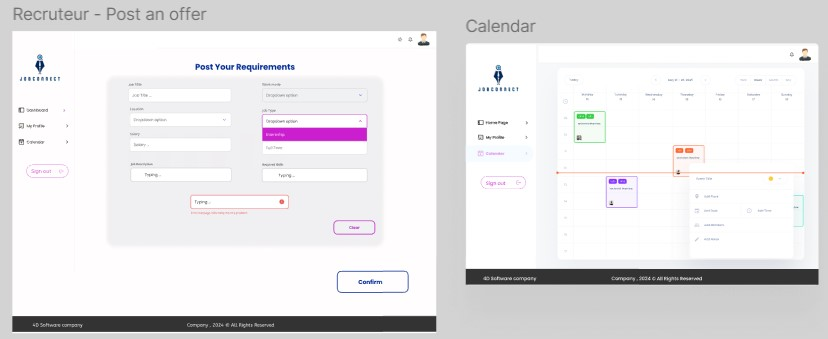
\includegraphics[scale=1.2]{Images/5.jpg} 
   \caption{Maquettes créer une offre et consulter calendrier}
   \label{fig:maquette5}
\end{figure}


\section{Architecture de l'application}
\subsection{Architecture physique}
% Notre application adopte une architecture client/serveur 
% multi-tiers. Ainsi, l'accès à 
% l'application nécessite le transit par des requêtes HTTP pour 
% récupérer et déposer les données dans le dépôt central. De plus, 
% nous avons centralisé la gestion de la base de données du système, 
% la séparant de la logique métier pour faciliter la maintenance. 
% Enfin, l'application est répartie sur plusieurs serveurs, chacun 
% responsable d'une tâche spécifique. Cette répartition des tâches 
% entre les serveurs permet d'assurer une grande souplesse, 
% des performances optimales et des temps de réponse rapides. 
Notre application adopte une architecture client/serveur multi-tiers. 
Les requêtes HTTP permettent de récupérer et déposer des données dans le dépôt 
central. La gestion de la base de données est centralisée et séparée de la 
logique métier pour faciliter la maintenance. L'application est répartie sur 
plusieurs serveurs, chacun responsable d'une tâche spécifique, assurant ainsi 
une rapidité de réponse.
La figure \ref{fig:physiqueArch} illustre l'architecture physique que nous avons mis en place :


\begin{figure}[htbp]
   \centering
   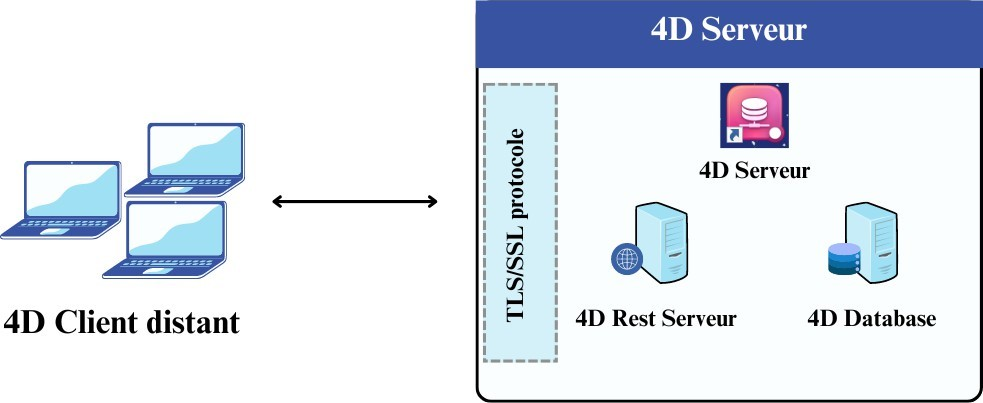
\includegraphics[scale=0.6]{Images/physique.jpg} % Replace with the actual filename of the IBM logo image
   \caption{Architecture physique}
   \label{fig:physiqueArch}
\end{figure}

Cette architecture se compose principalement des éléments suivants :
\begin{itemize}
   \item[•] \textbf{Serveur REST :} Un serveur web qui suit les principes de l’architecture REST et expose des ressources via des URIs, permettant aux clients d’effectuer des opérations standardisées sur ces ressources pour accéder aux données et fonctionnalités du serveur.
   \item[•] \textbf{Serveur 4D :} Ce serveur contient la couche métier de notre application.
   \item[•] \textbf{Serveur de base de données :} Ce serveur se charge de la gestion du stockage des données.
   \item[•] \textbf{Couche réseau :} Le protocole TLS sécurise les connexions client/serveur en cryptant les données échangées, permettant ainsi de renforcer la sécurité de l'application.
\end{itemize}

\subsection{Architecture logique}
% Pour avoir une architecture robuste, modulable et évolutive, il faut utiliser 
% le principe de « Couche », et donc séparer au maximum les différents types de 
% traitement de l’ap- plication. L’environnement de travail n’est pas dépendant 
% à une technologie spécifique. Pour cette raison, nous avons utilisé plusieurs 
% technologies afin de développer une solu- tion aboutie, performante, 
% multicouches et qui s’intègre parfaitement. La figure suivante illustre 
% l’architecture logicielle proposée pour le système développé, en présentant 
% trois couches : couche présentation (web), couche métier qui s’occupe des 
% différents traitements et couche accès aux données.

Notre application adopte une architecture composee des couches suivantes : la couche web, la couche metier et la couche ORDA

\begin{figure}[htbp]
   \centering
   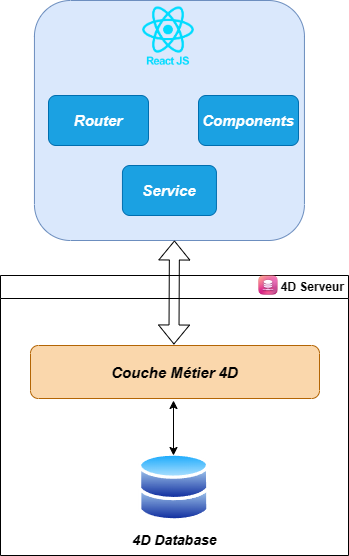
\includegraphics[scale=0.5]{Images/logi.png} 
   \caption{Architecture logique}
   \label{fig:logiqueArch}
\end{figure}

Au niveau 4D Server, notre développement s’est concentré principalement sur la couche métier. En effet, 4D Server offre un environnement de développement qui simplifie considérablement la création d’applications. Les autres couches, telles que la couche d’accès aux données et la couche de présentation, sont déjà implémentées et intégrées dans 4D.
\newline

Ainsi, les développeurs peuvent se concentrer sur la logique métier de leurs applications sans avoir à se soucier des détails techniques des autres couches. Cette approche permet un développement rapide et efficace, tout en offrant des fonctionnalités avancées pour répondre aux besoins spécifiques des projets.
\newline

% Aussi, nous avons travaillé avec ORDA, est une technologie spécifique qui facilite l’accès à une base de données relationnelle en tant qu’objets. Elle permet de manipuler les données de la base de données à l’aide d’un langage de programmation orienté objet ou d’interfaces utilisateur spécifiques. ORDA simplifie l’interaction avec la base de données en fournissant des abstractions supplémentaires et en masquant certaines complexités liées aux requêtes SQL.
% ORDA nous permet de créer des fonctions de classe de haut niveau au-dessus du modèle de données. Cela nous permet d’écrire du code orienté métier et de le «publier» comme une API. Le datastore, les
% dataclasses, les entity selections et les entités sont tous disponibles en tant qu’objets de classe pouvant contenir des fonctions.
Aussi, nous avons travaillé avec ORDA, une technologie qui facilite l’accès 
à la base de données 
relationnelle en tant qu’objets. 
Elle permet de manipuler les données de la base de données à l’aide d’un 
langage de programmation orienté objet. 
ORDA simplifie l’interaction avec la base de données en fournissant 
des abstractions supplémentaires et en masquant certaines complexités 
liées aux requêtes SQL.
\newline

% Grâce à 4D, les développeurs peuvent se concentrer sur l’essentiel et créer des appli- cations puissantes et performantes en toute simplicité.


% \begin{figure}[htbp]
%    \centering
%    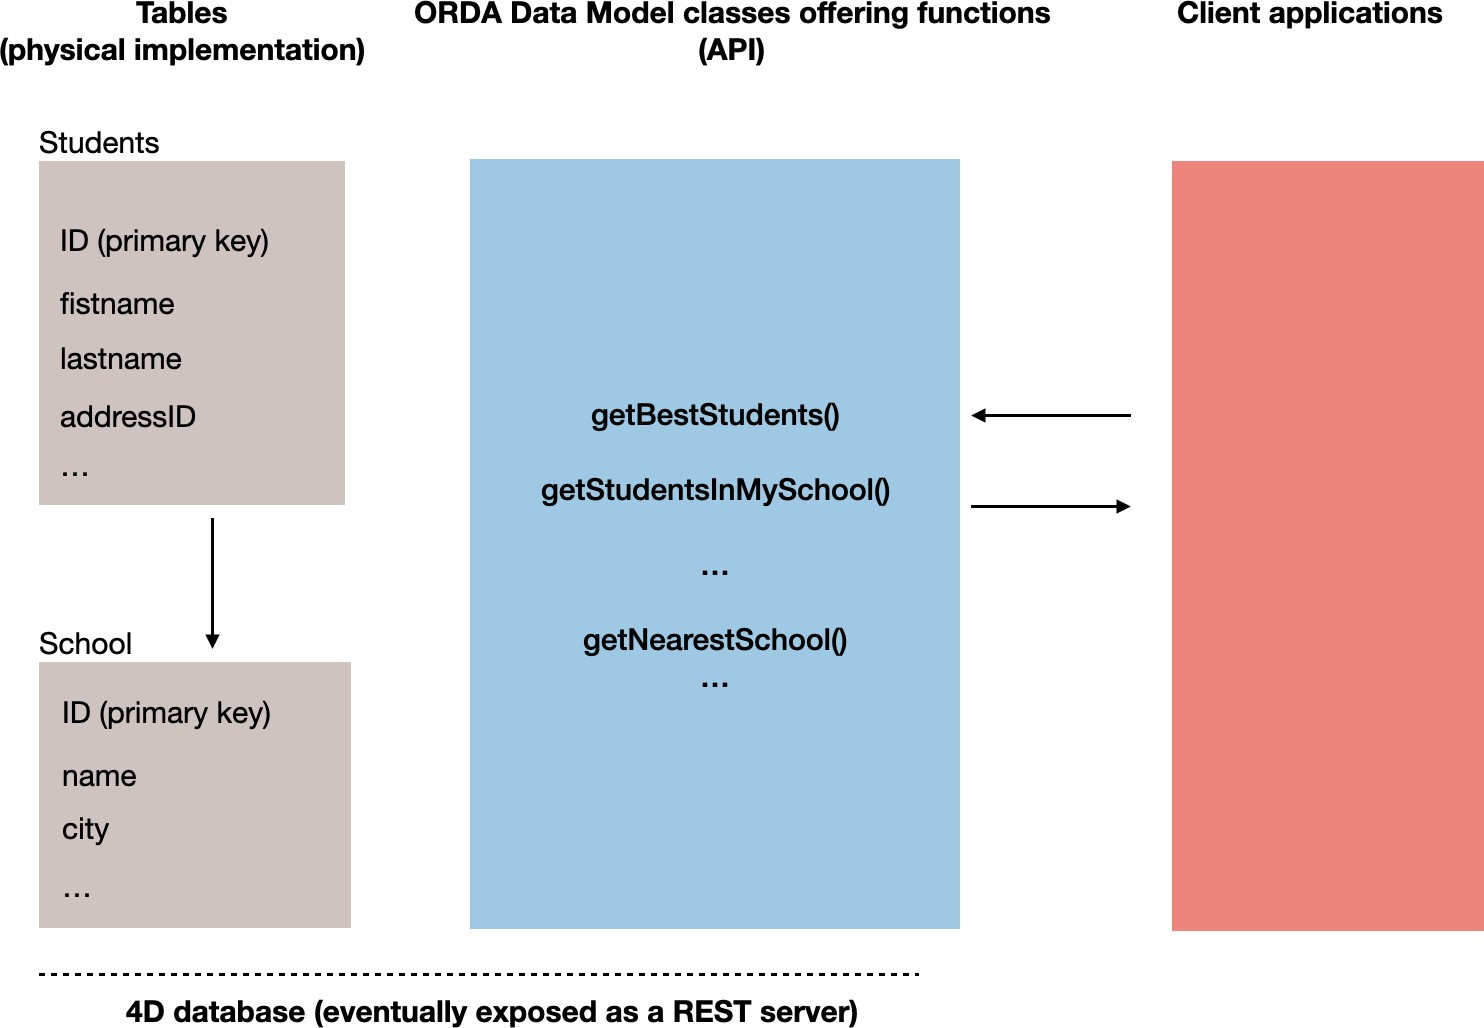
\includegraphics[scale=0.3]{Images/logique 2.jpg} 
%    \caption{Architecture logique}
%    \label{fig:logiqueArch}
% \end{figure}


% \subsection{Architecture technique}

% \begin{figure}[htbp]
%    \centering
%    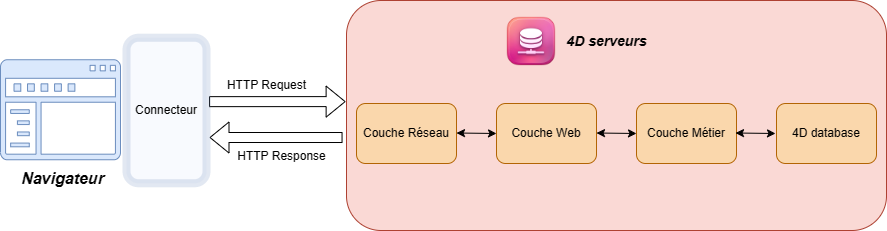
\includegraphics[scale=0.6]{Images/techn.png} % Replace with the actual filename of the IBM logo image
%    \caption{Architecture technique}
%    \label{fig:seq4}
% \end{figure}

% Le connecteur s’occupe de la récolte des données saisies par l’utilisateur dans le navi- gateur, ces données sont envoyées au serveur 4D via des requêtes HTTP. La couche web récupère les données reçues et les transmet à la couche métier qui effectue les traitements nécessaires. La couche 4D Database s’occupe de la sérialisation et la dé-sérialisation.

% \section{Conception détaillée}
\section{Diagramme de Classes}
Le diagramme de classes est l'un des diagrammes statiques d'UML. 
Il permet de représenter la structure d'un système informatique en 
présentant les différentes classes, leurs attributs, leurs méthodes, 
ainsi que les relations entre elles.

\begin{figure}[htbp]
   \centering
   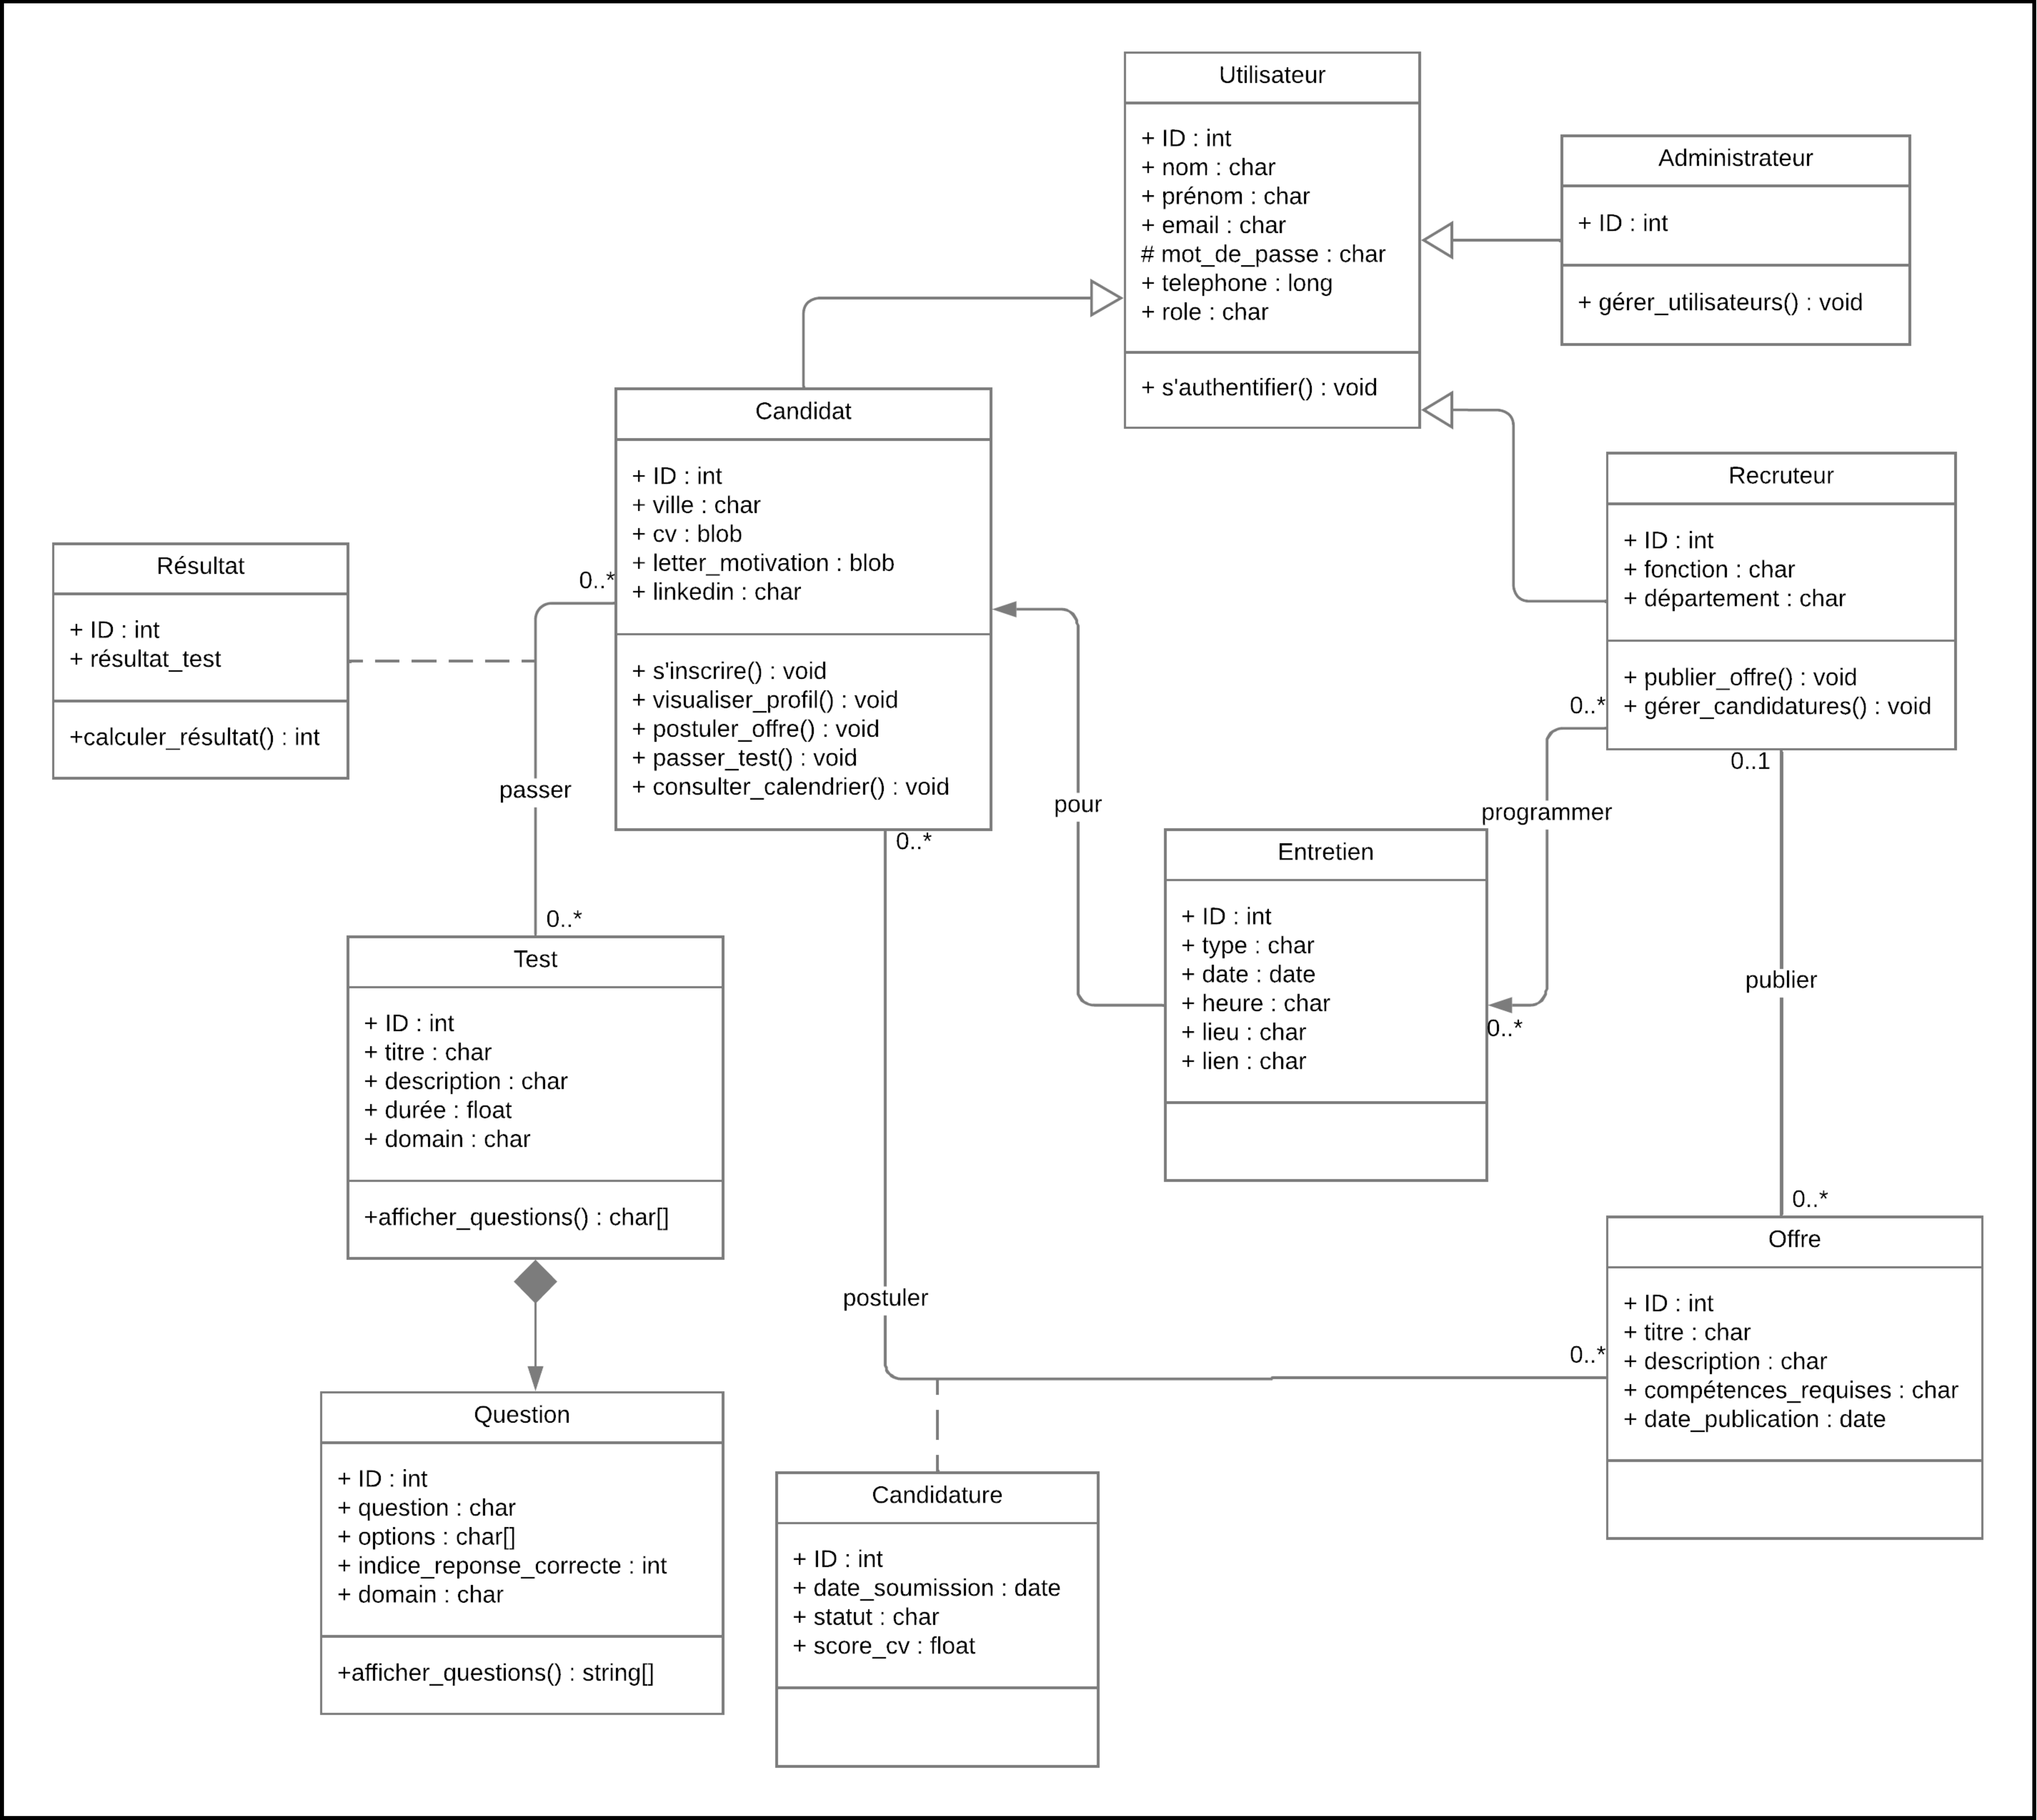
\includegraphics[scale=0.3]{Images/classDiagram.png} % Replace with the actual filename of the IBM logo image
   \caption{Diagramme de classes}
   \label{fig:ClassDiag}
\end{figure}
%commentaire !!!!



\section{Diagrammes de séquence}
Le diagramme de séquence offre une représentation claire 
et détaillée des interactions entre les divers objets ou 
composants d’un système. Dans le cadre de notre projet, 
ce diagramme nous permet de modéliser de manière précise et 
compréhensible les échanges entre les utilisateurs et l’interface 
utilisateur de l’application, ainsi que les interactions entre cette 
dernière, le serveur et la base de données associée.

\begin{figure}[htbp]
   \centering
   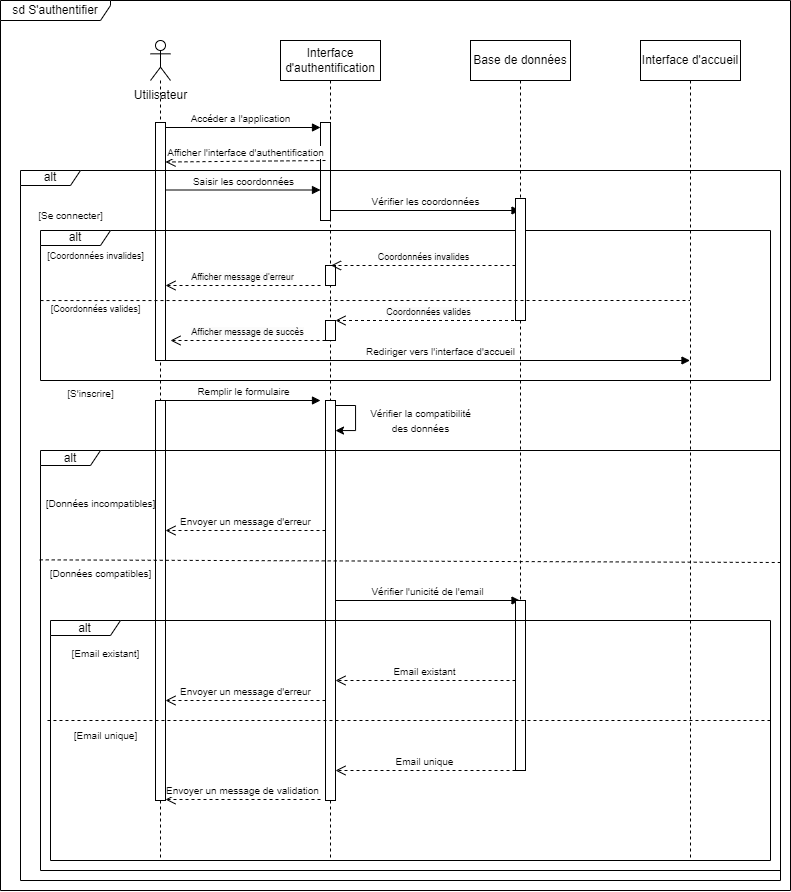
\includegraphics[scale=0.8]{Images/auth.png} % Replace with the actual filename of the IBM logo image
   \caption{Diagramme de séquence d’authentification}
   \label{fig:seq1}
\end{figure}

\begin{figure}[htbp]
   \centering
   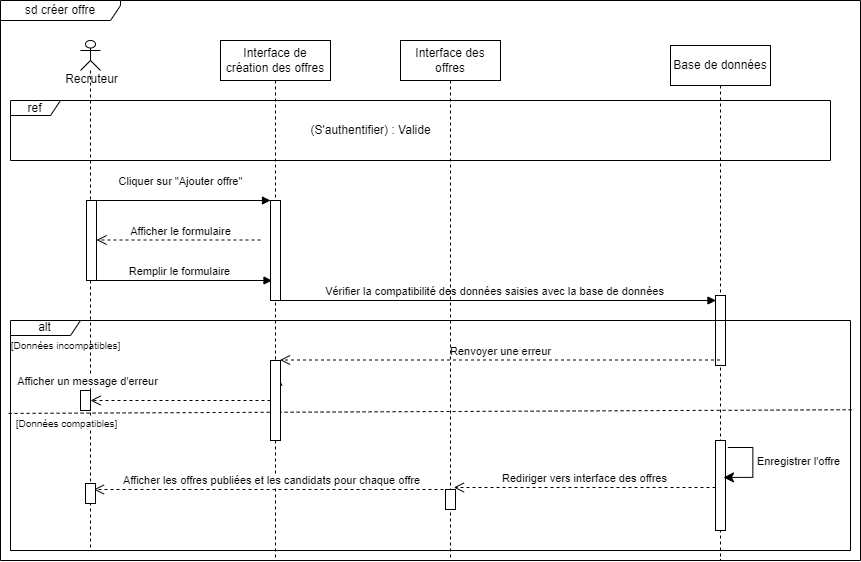
\includegraphics[scale=0.8]{Images/creerOffre.png} % Replace with the actual filename of the IBM logo image
   \caption{Diagramme de séquence de création des offres}
   \label{fig:seq2}
\end{figure}

\begin{figure}[htbp]
   \centering
   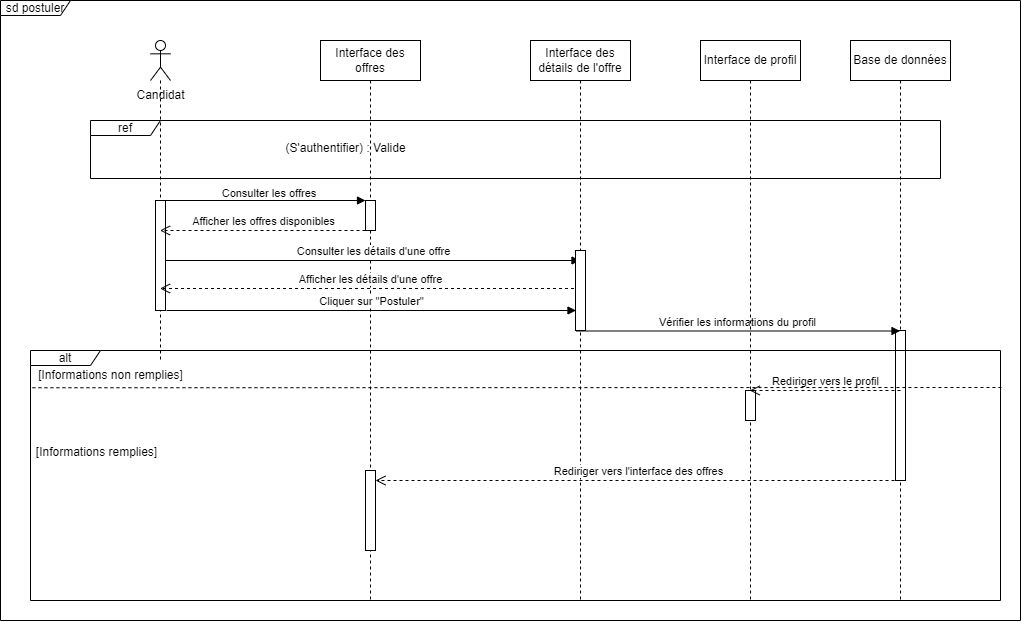
\includegraphics[scale=0.6]{Images/postuler.png} % Replace with the actual filename of the IBM logo image
   \caption{Diagramme de séquence de postulation}
   \label{fig:seq3}
\end{figure}

\begin{figure}[htbp]
   \centering
   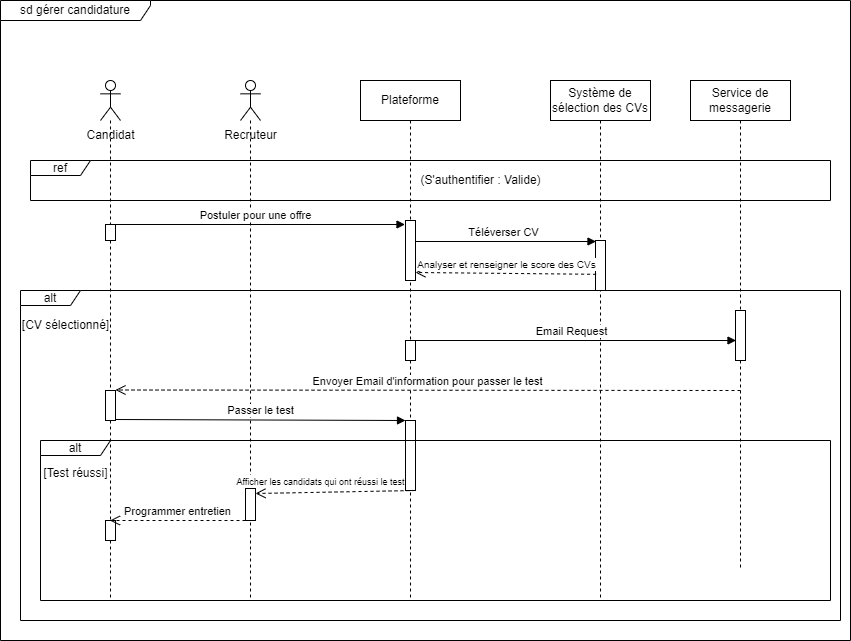
\includegraphics[scale=0.8]{Images/gererCandidature.png} % Replace with the actual filename of the IBM logo image
   \caption{ Diagramme de séquence de gestion des candidatures}
   \label{fig:seq4}
\end{figure}


\section{Conclusion}
Ce chapitre a présenté une conception 
de la solution. Nous avons d'abord 
élaboré les maquettes UX/UI pour aligner les attentes 
des utilisateurs finaux avec les fonctionnalités 
du système, puis nous avons décrit l'architecture 
physique en détaillant les serveurs et les couches 
réseau impliquées. Ensuite, l'architecture logique 
a été illustrée, mettant en avant l'utilisation de 
4D Server et ORDA pour simplifier le développement. 
Enfin, nous avons exposé les diagrammes de classes 
et de séquence de la solution.